\documentclass[12pt]{standalone}
\usepackage{tikz}
\usetikzlibrary{intersections} %calc, arrows.meta, decorations.pathreplacing}

\begin{document}

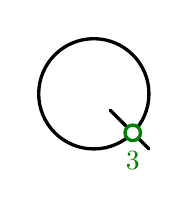
\begin{tikzpicture}[line width=1.2pt, line cap=round, line join=round, scale=1.4]
\path[name path=Qcirc, save path=\Qcirc] (0.5,0.5) circle(0.5);
\path[name path=Qtail, save path=\Qtail] (0.65,0.35) -- (1,0);
\path[name intersections={of=Qcirc and Qtail,by=Z}];
\begin{scope}[even odd rule]
\clip (-0.1, -0.1) rectangle (1.1, 1.1) (Z) circle(2pt);
\draw[use path=\Qcirc];
\draw[use path=\Qtail];
\end{scope}
\draw[green!50!black] (Z) circle(2pt) node[anchor=north, yshift=-3pt]{3};
\end{tikzpicture}
\end{document}
